\documentclass{beamer}
\usepackage{minted}
\usemintedstyle{default}


\begin{document}

\begin{frame}
\frametitle{Performance Optimisation}
\begin{itemize}
\item The same algorithm must be executed for each pixel.
\pause
\item Standard resolution: $1920 \times 1080 = 2073600$ pixels.
\pause
\item Parallel computing allows simultaneous program execution.
\pause
\item Multi-threading allows use of multiple CPU cores. On average CPU has 2-8 cores.
\end{itemize}
\end{frame}


\begin{frame}
\frametitle{The Graphics Processing Unit}
\begin{itemize}
\item Designed primarily for computer graphics.
\pause
\item Video games, computer aided design (CAD), machine learning.
\pause
\item GPUs have 1,000s - 10,000s of cores.
\pause
\item Graphics APIs such as OpenGL, Vulkan, Direct3D, Metal.
\pause
\item "Shaders" are programs that execute on the GPU.
\pause
\item OpenGL has bindings for many languages including Python (via PyOpenGL).
\pause
\item Used in conjunction with GUI library (GLUT, Tkinter via pyopengltk)
\end{itemize}
\end{frame}


\begin{frame}
\frametitle{OpenGL Rendering Pipeline}
\centering
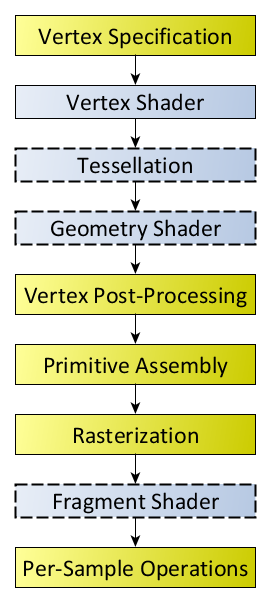
\includegraphics[width=0.3\textwidth]{RenderingPipeline.png}
\par \tiny {Source: https://www.khronos.org/opengl/wiki/Rendering\_Pipeline\_Overview}

\end{frame}


\begin{frame}[fragile]
\frametitle{Fragment Shader}

\begin{minted}[fontsize=\tiny]{glsl}
#version 330 core
uniform vec2 resolution;

out vec4 color;

vec2 f(vec2 c, vec2 z)
{
    return vec2(z.x*z.x - z.y*z.y, 2.0*z.x*z.y) + c;
}

void main()
{
    vec2 z = vec2(0.0, 0.0);
    vec2 coord = (((gl_FragCoord.xy - resolution.xy/2)/resolution.x) * 2.0);
    vec2 c = coord / 0.5;

    int max_iter = 128;
    int i = 0;
    while (i < max_iter && length(z) < 2.0)
    {
        z = f(c, z);
        ++i;
    }

    if (i == max_iter)
    {
        color = vec4(0.0, 0.0, 0.0, 1.0);
    } else {
        color = vec4(1.0, 1.0, 1.0, 1.0);
    }
}

\end{minted}

\end{frame}


\begin{frame}
\frametitle{Fragment Shader}
\centering

\includegraphics[width=1.0\textwidth]{GreyscaleMandelbrot.png}
\end{frame}

\begin{frame}[fragile]
\frametitle{Adding Colour}

\begin{minted}[fontsize=\tiny]{glsl}
#version 330 core
uniform vec2 resolution;

out vec4 color;

vec2 f(vec2 c, vec2 z)

vec3 HSV_to_RGB(vec3 col) {
    vec4 K = vec4(1.0, 2.0 / 3.0, 1.0 / 3.0, 3.0);
    vec3 p = abs(fract(col.xxx + K.xyz) * 6.0 - K.www);
    return col.z * mix(K.xxx, clamp(p - K.xxx, 0.0, 1.0), col.y);
}

void main()
{
    vec2 z = vec2(0.0, 0.0);
    vec2 coord = (((gl_FragCoord.xy - resolution.xy/2)/resolution.x) * 2.0);
    vec2 c = coord / 0.5;

    int max_iter = 128;
    int i = 0;
    while (i < max_iter && length(z) < 2.0)
    {
        z = f(c, z);
        ++i;
    }

    if (i == max_iter)
    {
        color = vec4(0.0, 0.0, 0.0, 1.0);
    } else {
        float t = float(i) / float(max_iter);
        color = vec4(HSV_to_RGB(vec3(t+0.6f, 1.0, 1.0)), 1.0);
    }
}

\end{minted}
\end{frame}


\begin{frame}
\frametitle{Adding Colour}

\includegraphics[width=1.0\textwidth]{ColourMandelbrot.png}
\end{frame}



\begin{frame}[fragile]
\frametitle{Adding Dynamic Visualisation}

\begin{minted}[fontsize=\tiny]{glsl}
#version 330 core
uniform vec2 resolution;
uniform vec2 L_pan;
uniform float scale;

out vec4 color;

vec2 f(vec2 c, vec2 z)
vec3 HSV_to_RGB(vec3 col)

void main()
{
    vec2 z = vec2(0.0, 0.0);
    vec2 coord = (((gl_FragCoord.xy - resolution.xy/2)/resolution.x) * 2.0);
    vec2 c = coord / scale + L_pan;

    int max_iter = 128;
    int i = 0;
    while (i < max_iter && length(z) < 2.0)
    {
        z = f(c, z);
        ++i;
    }

    if (i == max_iter)
    {
        color = vec4(0.0, 0.0, 0.0, 1.0);
    } else {
        float t = float(i) / float(max_iter);
        color = vec4(HSV_to_RGB(vec3(t+0.6f, 1.0, 1.0)), 1.0);
    }
}


\end{minted}
\end{frame}


\begin{frame}
\frametitle{Adding Dynamic Visualisation}

\includegraphics[width=1.0\textwidth]{ZoomedMandelbrot.png}
\par \tiny {Location: $-0.78 + 0.13i$}
\end{frame}


\begin{frame}[fragile]
\frametitle{Julia Sets}

\begin{minted}[fontsize=\tiny]{glsl}
#version 330 core
uniform vec2 resolution;
uniform vec2 L_pan;
uniform vec2 R_pan;
uniform float scale;

out vec4 color;

vec2 f(vec2 c, vec2 z)
vec3 HSV_to_RGB(vec3 col)

void main()
{
    vec2 c = L_pan;
    vec2 coord = (((gl_FragCoord.xy - resolution.xy/2)/resolution.x) * 2.0);
    vec2 z = coord / scale + R_pan;

    int max_iter = 128;
    int i = 0;
    while (i < max_iter && length(z) < 2.0)
    {
        z = f(c, z);
        ++i;
    }

    if (i == max_iter)
    {
        color = vec4(0.0, 0.0, 0.0, 1.0);
    } else {
        float t = float(i) / float(max_iter);
        color = vec4(HSV_to_RGB(vec3(t+0.6f, 1.0, 1.0)), 1.0);
    }
}

\end{minted}
\end{frame}


\begin{frame}
\frametitle{Julia Sets}
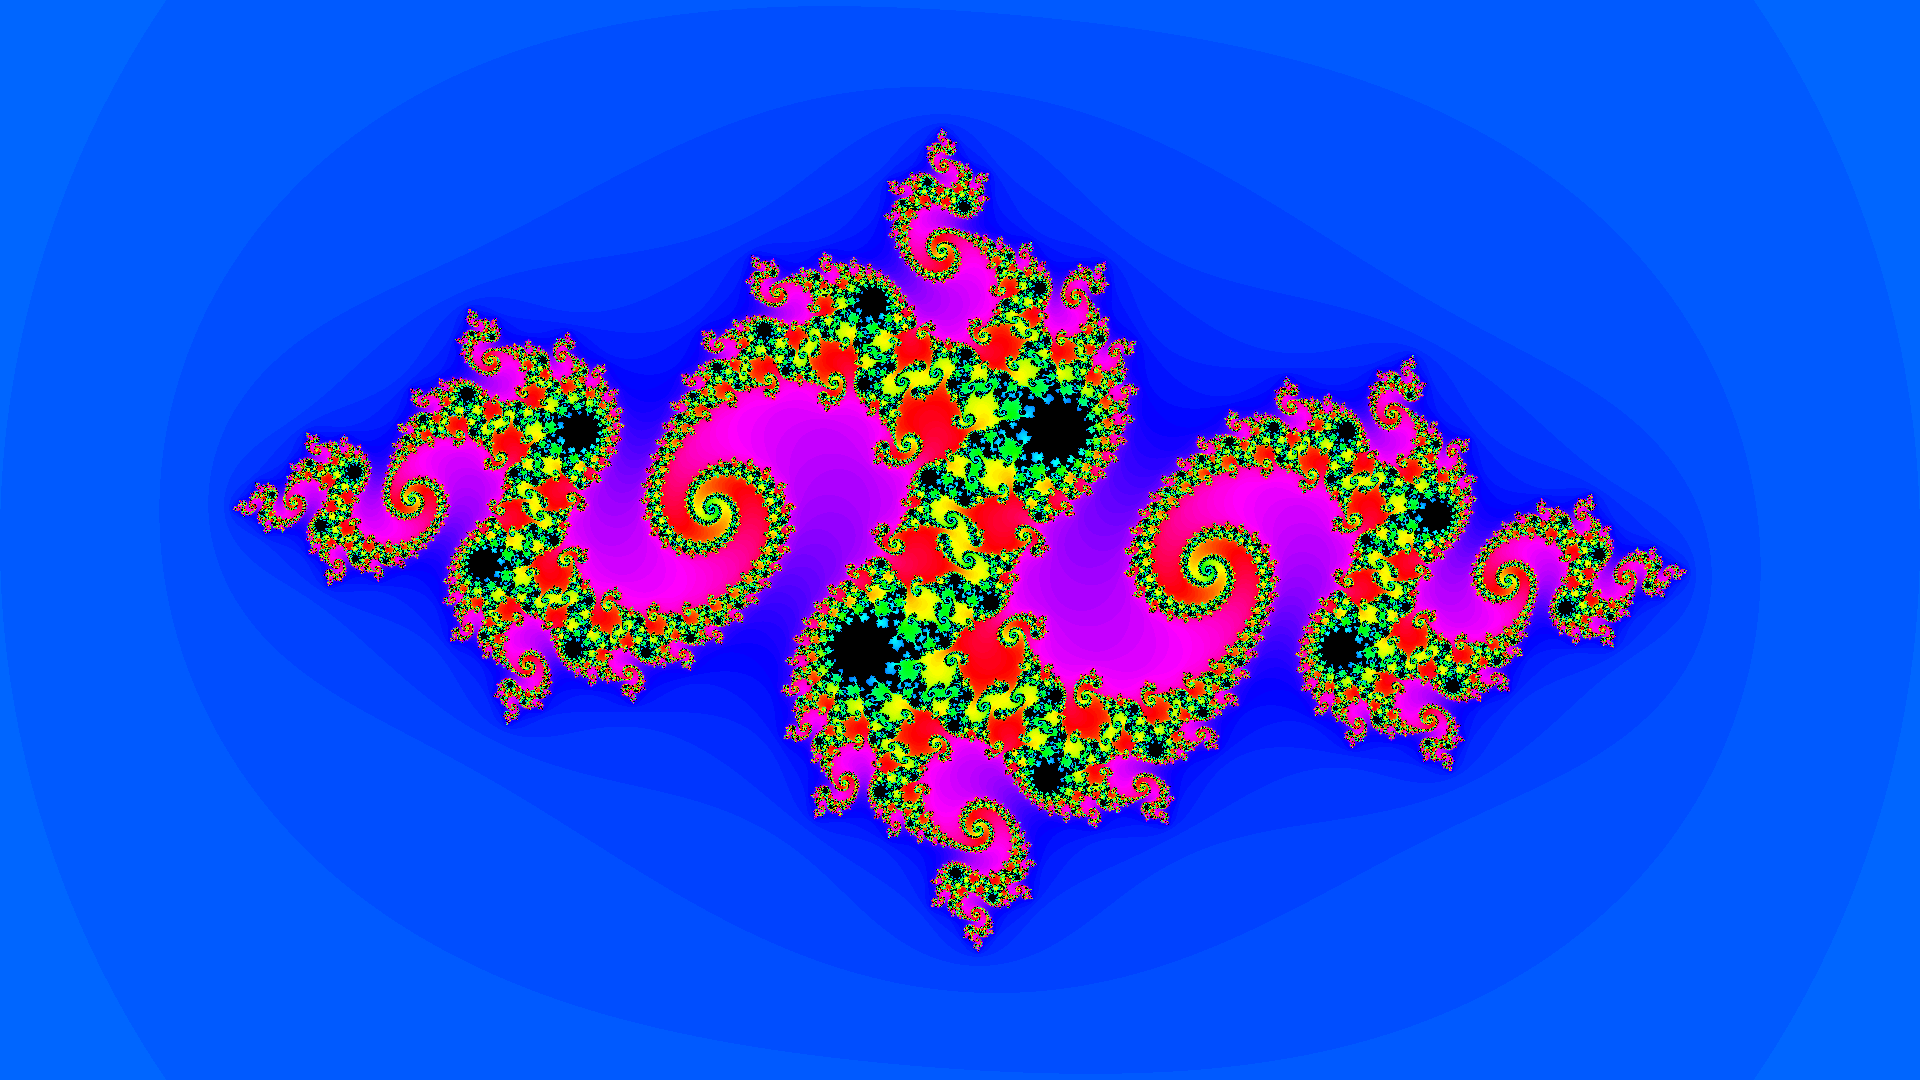
\includegraphics[width=1.0\textwidth]{Julia.png}
\par \tiny {Location: $0.78 + 0.13i$}
\end{frame}

\end{document}
